%\VignetteKeywords{genomation}
%\VignettePackage{genomation}
%\VignetteEngine{knitr::knitr}
%\VignetteIndexEntry{genomation: User Guide}
% !Rnw weave = knitr
\documentclass{article}\usepackage[]{graphicx}\usepackage[]{color}
%% maxwidth is the original width if it is less than linewidth
%% otherwise use linewidth (to make sure the graphics do not exceed the margin)
\makeatletter
\def\maxwidth{ %
  \ifdim\Gin@nat@width>\linewidth
    \linewidth
  \else
    \Gin@nat@width
  \fi
}
\makeatother

\definecolor{fgcolor}{rgb}{0.345, 0.345, 0.345}
\newcommand{\hlnum}[1]{\textcolor[rgb]{0.686,0.059,0.569}{#1}}%
\newcommand{\hlstr}[1]{\textcolor[rgb]{0.192,0.494,0.8}{#1}}%
\newcommand{\hlcom}[1]{\textcolor[rgb]{0.678,0.584,0.686}{\textit{#1}}}%
\newcommand{\hlopt}[1]{\textcolor[rgb]{0,0,0}{#1}}%
\newcommand{\hlstd}[1]{\textcolor[rgb]{0.345,0.345,0.345}{#1}}%
\newcommand{\hlkwa}[1]{\textcolor[rgb]{0.161,0.373,0.58}{\textbf{#1}}}%
\newcommand{\hlkwb}[1]{\textcolor[rgb]{0.69,0.353,0.396}{#1}}%
\newcommand{\hlkwc}[1]{\textcolor[rgb]{0.333,0.667,0.333}{#1}}%
\newcommand{\hlkwd}[1]{\textcolor[rgb]{0.737,0.353,0.396}{\textbf{#1}}}%

\usepackage{framed}
\makeatletter
\newenvironment{kframe}{%
 \def\at@end@of@kframe{}%
 \ifinner\ifhmode%
  \def\at@end@of@kframe{\end{minipage}}%
  \begin{minipage}{\columnwidth}%
 \fi\fi%
 \def\FrameCommand##1{\hskip\@totalleftmargin \hskip-\fboxsep
 \colorbox{shadecolor}{##1}\hskip-\fboxsep
     % There is no \\@totalrightmargin, so:
     \hskip-\linewidth \hskip-\@totalleftmargin \hskip\columnwidth}%
 \MakeFramed {\advance\hsize-\width
   \@totalleftmargin\z@ \linewidth\hsize
   \@setminipage}}%
 {\par\unskip\endMakeFramed%
 \at@end@of@kframe}
\makeatother

\definecolor{shadecolor}{rgb}{.97, .97, .97}
\definecolor{messagecolor}{rgb}{0, 0, 0}
\definecolor{warningcolor}{rgb}{1, 0, 1}
\definecolor{errorcolor}{rgb}{1, 0, 0}
\newenvironment{knitrout}{}{} % an empty environment to be redefined in TeX

\usepackage{alltt}
\usepackage{geometry}
\usepackage{wrapfig}

\geometry{verbose,tmargin=2.5cm,bmargin=2.5cm,lmargin=2.5cm,rmargin=2.5cm}


\title{\textbf{genomation} \\ a toolkit for annotation and visualization of genomic data}

\author{Altuna Akalin \\ \texttt{altuna.akalin@fmi.ch}
\and Vedran Franke \\ \texttt{vedran.franke@gmail.com} }


\newcommand{\Rpackage}[1]{{\textit{#1}}}
\newcommand{\Rcode}[1]{{\texttt{#1}}}
\newcommand{\Rclass}[1]{{\textit{#1}}}




\IfFileExists{upquote.sty}{\usepackage{upquote}}{}

\begin{document}
\maketitle
\tableofcontents
\vspace{300pt}

% ----------------------------------------------------------------- %
\section{Introduction}

\Rpackage{genomation}  is a  toolkit for annotation and in bulk visualization of
genomic features (scored or unscored) over predefined regions.
 The \textbf{genomic features} which the package can handle can 
be anything with a minimal information of chromosome, start and end. 
The features could have any length and most of the time they are 
\begin{wrapfigure}{r}{0.35\textwidth}
\vspace{-15pt}
  \begin{center}
    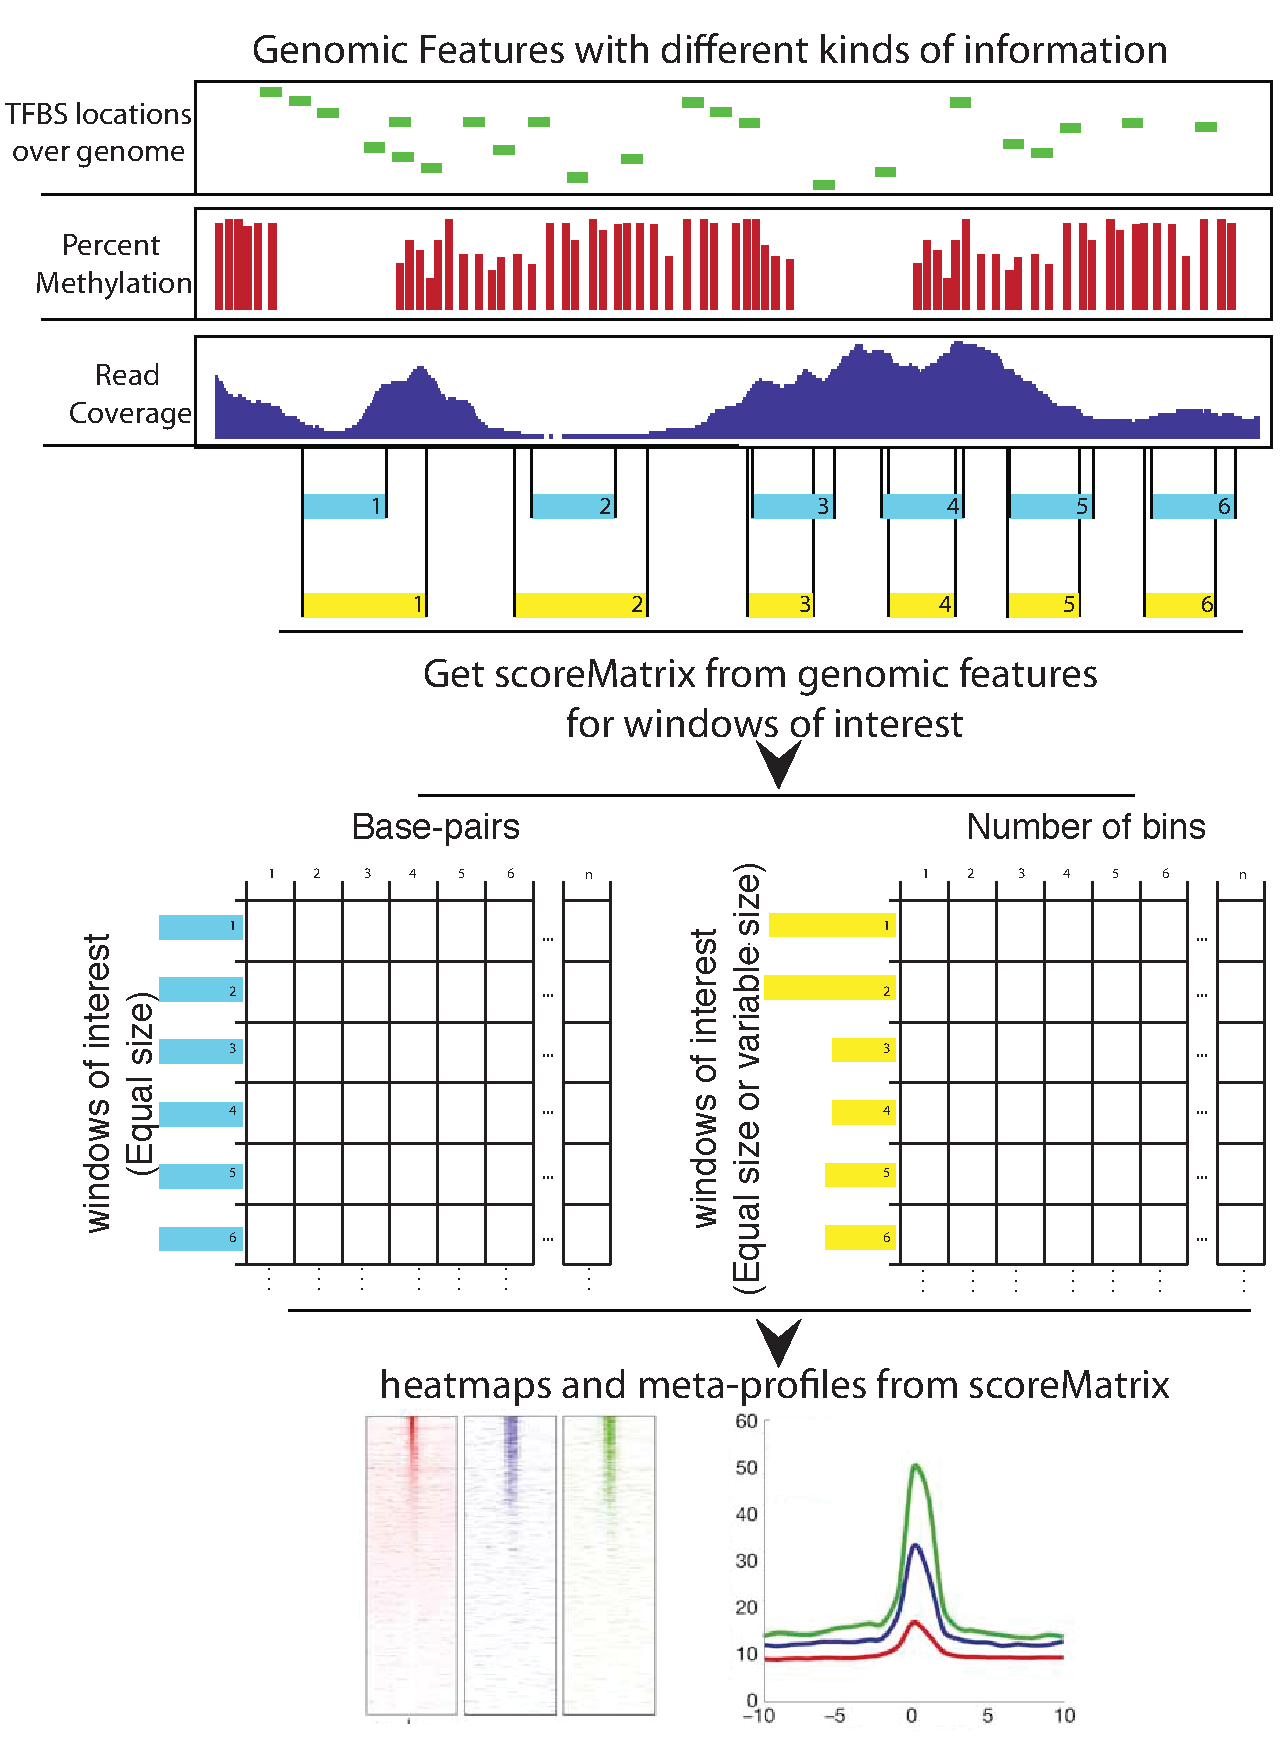
\includegraphics[width=0.35\textwidth]{Figures/genomationFlowChart1.pdf}
    \caption{Bulk visualization for different genomic feature datasets flowchart}
  \end{center}
  \vspace{-15pt}
\end{wrapfigure}
associated with a score. Typical examples of such data sets include aligned  
reads from high-throughput sequencing (HTS) experiments, percent methylation 
values for CpGs (or other cytosines), locations of transcription factor binding, 
and so on. On the other hand, throughout the vignette we use the phrase 
"genomic annotation" to refer to the regions of the genome associated with a 
potential function which does not necessarily have a score 
(examples: CpG islands, genes, enhancers, promoter, exons, etc. ). 
These genomic annotations are usually the regions of interest, and distribution 
of genomic features over/around the annotations are can make the way for 
biological interpretation of the data.
The pipeline for computational knowledge extraction consists of three steps: 
data filtering, integration of data from multiple sources or generation of 
predictive models and biological interpretation of produced models, which leads 
to novel hypotheses that can be tested in the wetlab. \Rpackage{genomation} aims
to facilitate the integration of multiple sources of genomic features with 
genomic annotation or already published experimental results.


% ----------------------------------------------------------------- %
\section{Access the data}

High-throughput data which will be used to show the functonality of the 
\Rpackage{genomation} are located in two places. The annotation and cap analysis
of gene expression (CAGE) data comes prepared with the genomation package, while
the raw HTS data can be found in the sister package \Rpackage{genomationData}.
To install the \Rpackage{genomation} and the complementary data package the from
the github repository c/p the following lines into your R interpreter:
\begin{knitrout}
\definecolor{shadecolor}{rgb}{0.969, 0.969, 0.969}\color{fgcolor}\begin{kframe}
\begin{alltt}
\hlkwd{library}\hlstd{(devtools)}
\hlkwd{install_github}\hlstd{(}\hlstr{"genomationData"}\hlstd{,} \hlkwc{username} \hlstd{=} \hlstr{"al2na"}\hlstd{)}
\hlkwd{install_github}\hlstd{(}\hlstr{"genomation"}\hlstd{,} \hlkwc{username} \hlstd{=} \hlstr{"al2na"}\hlstd{)}
\end{alltt}
\end{kframe}
\end{knitrout}


The \Rpackage{genomationData} vignette contains a verbose description of 
included files. 
To list the available data, type:
\begin{knitrout}
\definecolor{shadecolor}{rgb}{0.969, 0.969, 0.969}\color{fgcolor}\begin{kframe}
\begin{alltt}
\hlkwd{list.files}\hlstd{(}\hlkwd{system.file}\hlstd{(}\hlstr{"extdata"}\hlstd{,} \hlkwc{package} \hlstd{=} \hlstr{"genomationData"}\hlstd{))}
\end{alltt}
\end{kframe}
\end{knitrout}


To see the descriptions of the files:
\begin{knitrout}
\definecolor{shadecolor}{rgb}{0.969, 0.969, 0.969}\color{fgcolor}\begin{kframe}
\begin{alltt}
\hlstd{sampleInfo} \hlkwb{<-} \hlkwd{read.table}\hlstd{(}\hlkwd{system.file}\hlstd{(}\hlstr{"extdata/SamplesInfo.txt"}\hlstd{,}
    \hlkwc{package} \hlstd{=} \hlstr{"genomationData"}\hlstd{),} \hlkwc{header} \hlstd{= T,} \hlkwc{sep} \hlstd{=} \hlstr{"\textbackslash{}t"}\hlstd{)}
\hlkwd{head}\hlstd{(sampleInfo)}
\end{alltt}
\end{kframe}
\end{knitrout}


Basic annotation data and processed experimental data can be found within the 
\Rpackage{genomation} package.
The data can be accesed throught the \Rcode{data} command or located 
in the extdata folder. 
\begin{knitrout}
\definecolor{shadecolor}{rgb}{0.969, 0.969, 0.969}\color{fgcolor}\begin{kframe}
\begin{alltt}
\hlkwd{library}\hlstd{(genomation)}
\hlkwd{data}\hlstd{(cage)}
\hlkwd{data}\hlstd{(cpgi)}

\hlkwd{list.files}\hlstd{(}\hlkwd{system.file}\hlstd{(}\hlstr{"extdata"}\hlstd{,} \hlkwc{package} \hlstd{=} \hlstr{"genomation"}\hlstd{))}
\end{alltt}
\end{kframe}
\end{knitrout}




% ----------------------------------------------------------------- %
\section{Data input}

One of larger hindrances in computational genomics stems from the myriad of 
formats that are used to store the data. Although some formats have been 
selected as de facto standards for specific kind of biological data (e.g. BAM, VCF), 
almost all publications come with supplementary tables that do not have the 
same structure, but hold similar information. The tables usually have a tabular 
format, contain the locationof elements in genomic coordinates and various 
metadata colums. \Rpackage(genomation) contais functions to read genomic 
features and genomic annotation provided they are in a tabular format. 
These functions will read the data from flat files into GRanges or GRangesList 
objects.

\Rcode{readGeneric} is the workhorse of the genomation package. It is a function
developed specifically for input of genomic data in tabular formats, and their 
conversion to a GRanges object. 
By default, the function persumes that the file is a standard .bed file 
containing columns chr, start, end.
\begin{knitrout}
\definecolor{shadecolor}{rgb}{0.969, 0.969, 0.969}\color{fgcolor}\begin{kframe}
\begin{alltt}
\hlkwd{library}\hlstd{(genomation)}
\hlstd{tab.file1} \hlkwb{<-} \hlkwd{system.file}\hlstd{(}\hlstr{"extdata/tab1.bed"}\hlstd{,} \hlkwc{package} \hlstd{=} \hlstr{"genomation"}\hlstd{)}
\hlkwd{readGeneric}\hlstd{(tab.file1)}
\end{alltt}
\end{kframe}
\end{knitrout}


If the file contains meta data columns (as in extended bed format), 
it is possible to read all or some of the additional columns.
To select columns which you want to read in, use the \Rcode{meta.col} argument 
\begin{knitrout}
\definecolor{shadecolor}{rgb}{0.969, 0.969, 0.969}\color{fgcolor}\begin{kframe}
\begin{alltt}
\hlkwd{readGeneric}\hlstd{(tab.file1,} \hlkwc{keep.all.metadata} \hlstd{=} \hlnum{TRUE}\hlstd{)}

\hlkwd{readGeneric}\hlstd{(tab.file1,} \hlkwc{meta.col} \hlstd{=} \hlkwd{list}\hlstd{(}\hlkwc{CpGnum} \hlstd{=} \hlnum{4}\hlstd{))}
\end{alltt}
\end{kframe}
\end{knitrout}


If the file contains header, the function will automatically recognize the 
columns using the header names.
\begin{knitrout}
\definecolor{shadecolor}{rgb}{0.969, 0.969, 0.969}\color{fgcolor}\begin{kframe}
\begin{alltt}
\hlkwd{readGeneric}\hlstd{(tab.file1,} \hlkwc{header} \hlstd{=} \hlnum{TRUE}\hlstd{,} \hlkwc{keep.all.metadata} \hlstd{=} \hlnum{TRUE}\hlstd{)}
\end{alltt}
\end{kframe}
\end{knitrout}



If the files have permutted columns, such that the first three do not represent
chromosome, start and end, you can select an arbitrary set of columns using the
chr, start and end arguments.
\begin{knitrout}
\definecolor{shadecolor}{rgb}{0.969, 0.969, 0.969}\color{fgcolor}\begin{kframe}
\begin{alltt}
\hlstd{tab.file2} \hlkwb{<-} \hlkwd{system.file}\hlstd{(}\hlstr{"extdata/tab2.bed"}\hlstd{,} \hlkwc{package} \hlstd{=} \hlstr{"genomation"}\hlstd{)}
\hlkwd{readGeneric}\hlstd{(tab.file2,} \hlkwc{chr} \hlstd{=} \hlnum{3}\hlstd{,} \hlkwc{start} \hlstd{=} \hlnum{2}\hlstd{,} \hlkwc{end} \hlstd{=} \hlnum{1}\hlstd{)}
\end{alltt}
\end{kframe}
\end{knitrout}


\Rcode{readGeneric} function can easily be extended to read almost any kind of 
biological data. As an example we have provided convenience functions to read 
the Encode \Rcode{narrowPeak} and \Rcode{broadPeak} formats, and gtf formatted files.
\begin{knitrout}
\definecolor{shadecolor}{rgb}{0.969, 0.969, 0.969}\color{fgcolor}\begin{kframe}
\begin{alltt}
\hlstd{gff.file} \hlkwb{<-} \hlkwd{system.file}\hlstd{(}\hlstr{"extdata/chr21.refseq.hg19.gtf"}\hlstd{,}
    \hlkwc{package} \hlstd{=} \hlstr{"genomation"}\hlstd{)}
\hlstd{gff} \hlkwb{<-} \hlkwd{gffToGRanges}\hlstd{(gff.file)}
\hlkwd{head}\hlstd{(gff)}
\end{alltt}
\end{kframe}
\end{knitrout}


In order to split the last column of the gff file, use the 
\Rcode{split.group=TRUE} argument.
\begin{knitrout}
\definecolor{shadecolor}{rgb}{0.969, 0.969, 0.969}\color{fgcolor}\begin{kframe}
\begin{alltt}
\hlstd{gff} \hlkwb{<-} \hlkwd{gffToGRanges}\hlstd{(gff.file,} \hlkwc{split.group} \hlstd{=} \hlnum{TRUE}\hlstd{)}
\hlkwd{head}\hlstd{(gff)}
\end{alltt}
\end{kframe}
\end{knitrout}


There are specific functions to read genomic annotation from flat bed files.
\Rcode{readFeatureFlank} is a convenience function used to get the ranges flanking 
the set of interest. As an example, it could be used to get the CpG island shores, 
which have been shown to harbour condition specific differential methylation.
\begin{knitrout}
\definecolor{shadecolor}{rgb}{0.969, 0.969, 0.969}\color{fgcolor}\begin{kframe}
\begin{alltt}
\hlcom{# reading genes stored as a BED files}
\hlstd{cpgi.file} \hlkwb{<-} \hlkwd{system.file}\hlstd{(}\hlstr{"extdata/chr21.CpGi.hg19.bed"}\hlstd{,}
    \hlkwc{package} \hlstd{=} \hlstr{"genomation"}\hlstd{)}
\hlstd{cpgi.flanks} \hlkwb{<-} \hlkwd{readFeatureFlank}\hlstd{(cpgi.file)}
\hlkwd{head}\hlstd{(cpgi.flanks}\hlopt{$}\hlstd{flanks)}
\end{alltt}
\end{kframe}
\end{knitrout}




\begin{knitrout}
\definecolor{shadecolor}{rgb}{0.969, 0.969, 0.969}\color{fgcolor}\begin{kframe}
\begin{alltt}
\hlkwd{readGeneFeatures}\hlstd{()}
\end{alltt}
\end{kframe}
\end{knitrout}



% ----------------------------------------------------------------- %
\section{Extraction and visualization of genomic data}

A standard step in a computational genomics experiment is visualization of 
average enrichment over a certain predefined set of ranges, such as mean coverage
of a certain histone modification around a transcription factor binding site,
or visualization of histone positions around transcription start sites.


\subsection{Extration of data over genomic winows}

\Rcode{ScoreMatrix} and \Rcode{ScoreMatrixBin} are functions used to extract 
data over predefined windows.

\Rcode{ScoreMatrix} is used when all of the windows
have the same width, such as a designated area around the transcription start
site, while the \Rcode{ScoreMatrixBin} is designed for use with windows of 
unequal width (e.g. enrichment of methylation over exons).

Both functions have 2 main arguments: \Rcode{target} and 
\Rcode{windows}. \Rcode{target} is the data that we want to extract, while the 
\Rcode{windows} represents the regions over which we want to see the enrichment.
The target data can be in 3 forms: a GRanges, a RLeList or a path to an indexed 
.bam file. The \Rcode{windows} must be GRanges object.

As an example we will extract the density of cage tags around the promoters on 
the human chromosome 21.
\begin{knitrout}
\definecolor{shadecolor}{rgb}{0.969, 0.969, 0.969}\color{fgcolor}\begin{kframe}
\begin{alltt}
\hlkwd{data}\hlstd{(cage)}
\hlkwd{data}\hlstd{(promoters)}
\hlstd{sm} \hlkwb{<-} \hlkwd{ScoreMatrix}\hlstd{(}\hlkwc{target} \hlstd{= cage,} \hlkwc{windows} \hlstd{= promoters)}
\hlstd{sm}
\end{alltt}


{\ttfamily\noindent\itshape\color{messagecolor}{\#\#\ \  scoreMatrix with dims: 1055 2001}}\end{kframe}
\end{knitrout}



\Rcode{ScoreMatrixBin} function has an additional \Rcode{bin.num} argument which
specifies the number of bins that will represent each windot window  
(ie. it converts windows of unequal width into ones of equal width.). 
By default, the binning function is set
to \Rcode{mean}.
\begin{knitrout}
\definecolor{shadecolor}{rgb}{0.969, 0.969, 0.969}\color{fgcolor}\begin{kframe}
\begin{alltt}
\hlkwd{data}\hlstd{(cage)}
\hlstd{gff.file} \hlkwb{<-} \hlkwd{system.file}\hlstd{(}\hlstr{"extdata/chr21.refseq.hg19.gtf"}\hlstd{,}
    \hlkwc{package} \hlstd{=} \hlstr{"genomation"}\hlstd{)}
\hlstd{exons} \hlkwb{<-} \hlkwd{gffToGRanges}\hlstd{(gff.file,} \hlkwc{filter} \hlstd{=} \hlstr{"exon"}\hlstd{)}
\end{alltt}


{\ttfamily\noindent\itshape\color{messagecolor}{\#\# Filtering exon features...}}\begin{alltt}
\hlstd{sm} \hlkwb{<-} \hlkwd{ScoreMatrixBin}\hlstd{(}\hlkwc{target} \hlstd{= cage,} \hlkwc{windows} \hlstd{= exons,}
    \hlkwc{bin.num} \hlstd{=} \hlnum{50}\hlstd{)}
\end{alltt}


{\ttfamily\noindent\color{warningcolor}{\#\# Warning: supplied GRanges object contains ranges of width < number of bins}}\begin{alltt}
\hlstd{sm}
\end{alltt}


{\ttfamily\noindent\itshape\color{messagecolor}{\#\#\ \  scoreMatrix with dims: 5127 50}}\end{kframe}
\end{knitrout}


Running \Rcode{ScoreMatrixBin} with \Rcode{bin.num=50} on 
a set of exons warned us that some of the exons are shorter than 50 bp and
were thus removed from the set before binning. 
The rownames of the resulting \Rcode{ScoreMatrix} object correspond
to the ranges that were used to construct the windows (e.g. row name 10 means 
that the 10th element in the target GRanges object was used to extract the data). 
If a certain rowname is not present in the ScoreMatrix object, that means that 
the corresponding range was filtered out (e.g. the range could have been on a 
chromosome that was not present in the target).

To simultaneously work on multiple files you can use the \Rcode{ScoreMatrixList}
function. The function also has 2 obligatory arguments \Rcode{targets} and 
\Rcode{windows}. While the \Rcode{windows} is the same as in \Rcode{ScoreMatrix}, 
the targets argument contains results from multiple experiments. 
It can be in one of the three formats: a list of RleLists, a list of GRanges 
(or a GRangesList object), or a character vector designating a set of 
.bam or .bigWig files.
\begin{knitrout}
\definecolor{shadecolor}{rgb}{0.969, 0.969, 0.969}\color{fgcolor}\begin{kframe}
\begin{alltt}
\hlkwd{data}\hlstd{(promoters)}
\hlkwd{data}\hlstd{(cpgi)}
\hlkwd{data}\hlstd{(cage)}

\hlstd{cage}\hlopt{$}\hlstd{tpm} \hlkwb{<-} \hlkwa{NULL}
\hlstd{targets} \hlkwb{<-} \hlkwd{list}\hlstd{(}\hlkwc{cage} \hlstd{= cage,} \hlkwc{cpgi} \hlstd{= cpgi)}
\hlstd{sm} \hlkwb{<-} \hlkwd{ScoreMatrixList}\hlstd{(}\hlkwc{targets} \hlstd{= targets,} \hlkwc{windows} \hlstd{= promoters,}
    \hlkwc{bin.num} \hlstd{=} \hlnum{50}\hlstd{)}
\end{alltt}


{\ttfamily\noindent\itshape\color{messagecolor}{\#\# working on: cage\\\#\# working on: cpgi}}\begin{alltt}
\hlstd{sm}
\end{alltt}


{\ttfamily\noindent\itshape\color{messagecolor}{\#\# scoreMatrixlist of length:2\\\#\# \\\#\# 1. scoreMatrix with dims: 1055 50\\\#\# 2. scoreMatrix with dims: 1055 50}}\end{kframe}
\end{knitrout}


If all of the windows have the same width \Rcode{ScoreMatrixList} will use the
\Rcode{ScoreMatrix} function. That can be overridden by explicitly specifying the 
\Rcode{bin.num} argument, as we did in the example.


\subsection{Visualization of multiple genomic experiments}

There are 2 basic modes of visualization of enrichment over windows: either 
as a heatmap, or as a histogram. \Rcode{heatMatrix]}, \Rcode{plotMeta} and 
\Rcode{multiHeatMatrix} are functions for visualization of \Rcode{ScoreMatrix} 
and \Rcode{ScoreMatrixList} objects.

We will plot the distribution of CAGE tags around promoters on human chr21.

\begin{knitrout}
\definecolor{shadecolor}{rgb}{0.969, 0.969, 0.969}\color{fgcolor}\begin{kframe}
\begin{alltt}
\hlkwd{data}\hlstd{(cage)}
\hlkwd{data}\hlstd{(promoters)}
\hlstd{sm} \hlkwb{<-} \hlkwd{ScoreMatrix}\hlstd{(}\hlkwc{target} \hlstd{= cage,} \hlkwc{windows} \hlstd{= promoters)}

\hlstd{oldmar} \hlkwb{<-} \hlkwd{par}\hlstd{()}\hlopt{$}\hlstd{mar}
\hlkwd{par}\hlstd{(}\hlkwc{oma} \hlstd{=} \hlkwd{c}\hlstd{(}\hlnum{0}\hlstd{,} \hlnum{0}\hlstd{,} \hlnum{0}\hlstd{,} \hlnum{0}\hlstd{))}
\hlkwd{heatMatrix}\hlstd{(sm,} \hlkwc{xcoords} \hlstd{=} \hlkwd{c}\hlstd{(}\hlopt{-}\hlnum{1000}\hlstd{,} \hlnum{1000}\hlstd{))}
\hlkwd{plotMeta}\hlstd{(sm,} \hlkwc{xcoords} \hlstd{=} \hlkwd{c}\hlstd{(}\hlopt{-}\hlnum{1000}\hlstd{,} \hlnum{1000}\hlstd{))}
\hlkwd{par}\hlstd{(}\hlkwc{oma} \hlstd{= oldmar)}
\end{alltt}
\end{kframe}

{\centering \includegraphics[width=\maxwidth]{FiguresheatMatrix11} 
\includegraphics[width=\maxwidth]{FiguresheatMatrix12} 

}



\end{knitrout}


The \Rcode{heatMatrix} function can also take a list of numeric vectors 
designating row names, or a factor variable that represent our 
annotation over the windows.
\begin{knitrout}
\definecolor{shadecolor}{rgb}{0.969, 0.969, 0.969}\color{fgcolor}\begin{kframe}
\begin{alltt}
\hlkwd{data}\hlstd{(cage)}
\hlkwd{data}\hlstd{(promoters)}
\hlkwd{data}\hlstd{(cpgi)}

\hlstd{sm} \hlkwb{<-} \hlkwd{ScoreMatrix}\hlstd{(}\hlkwc{target} \hlstd{= cage,} \hlkwc{windows} \hlstd{= promoters,}
    \hlkwc{strand.aware} \hlstd{=} \hlnum{TRUE}\hlstd{)}
\hlstd{cpg.ind} \hlkwb{<-} \hlkwd{which}\hlstd{(}\hlkwd{countOverlaps}\hlstd{(promoters, cpgi)} \hlopt{>} \hlnum{0}\hlstd{)}
\hlstd{nocpg.ind} \hlkwb{<-} \hlkwd{which}\hlstd{(}\hlkwd{countOverlaps}\hlstd{(promoters, cpgi)} \hlopt{==}
    \hlnum{0}\hlstd{)}
\hlkwd{heatMatrix}\hlstd{(sm,} \hlkwc{xcoords} \hlstd{=} \hlkwd{c}\hlstd{(}\hlopt{-}\hlnum{1000}\hlstd{,} \hlnum{1000}\hlstd{),} \hlkwc{group} \hlstd{=} \hlkwd{list}\hlstd{(}\hlkwc{CpGi} \hlstd{= cpg.ind,}
    \hlkwc{noCpGi} \hlstd{= nocpg.ind))}

\hlcom{# cpg.ind = factor(countOverlaps(promoters,}
\hlcom{# cpgi)>0, levels=c('CpG','noCpG')) heatMatrix(sm,}
\hlcom{# xcoords=c(-1000, 1000), group=cpg.ind)}
\end{alltt}
\end{kframe}

{\centering \includegraphics[width=\maxwidth]{FiguresheatMatrix2} 

}



\end{knitrout}


Because the enrichment in windows can have a high dynamic range, it is sometimes
convenient to scale the matrix before plotting.
\begin{knitrout}
\definecolor{shadecolor}{rgb}{0.969, 0.969, 0.969}\color{fgcolor}\begin{kframe}
\begin{alltt}
\hlstd{sm.scaled} \hlkwb{<-} \hlkwd{scaleScoreMatrix}\hlstd{(sm)}
\hlkwd{heatMatrix}\hlstd{(sm.scaled,} \hlkwc{xcoords} \hlstd{=} \hlkwd{c}\hlstd{(}\hlopt{-}\hlnum{1000}\hlstd{,} \hlnum{1000}\hlstd{),} \hlkwc{group} \hlstd{=} \hlkwd{list}\hlstd{(}\hlkwc{CpGi} \hlstd{= cpg.ind,}
    \hlkwc{noCpGi} \hlstd{= nocpg.ind))}
\end{alltt}
\end{kframe}

{\centering \includegraphics[width=\maxwidth]{FiguresheatMatrixScales} 

}



\end{knitrout}



Several experiments can be plotted in a side by side fashion using a combination
of ScoreMatrixList and multiHeatMatrix.
\begin{knitrout}
\definecolor{shadecolor}{rgb}{0.969, 0.969, 0.969}\color{fgcolor}\begin{kframe}
\begin{alltt}
\hlstd{cage}\hlopt{$}\hlstd{tpm} \hlkwb{<-} \hlkwa{NULL}
\hlstd{targets} \hlkwb{<-} \hlkwd{list}\hlstd{(}\hlkwc{cage} \hlstd{= cage,} \hlkwc{cpgi} \hlstd{= cpgi)}
\hlstd{sml} \hlkwb{<-} \hlkwd{ScoreMatrixList}\hlstd{(}\hlkwc{targets} \hlstd{= targets,} \hlkwc{windows} \hlstd{= promoters,}
    \hlkwc{bin.num} \hlstd{=} \hlnum{50}\hlstd{,} \hlkwc{strand.aware} \hlstd{=} \hlnum{TRUE}\hlstd{)}
\end{alltt}


{\ttfamily\noindent\itshape\color{messagecolor}{\#\# working on: cage\\\#\# working on: cpgi}}\begin{alltt}
\hlkwd{multiHeatMatrix}\hlstd{(sml,} \hlkwc{xcoords} \hlstd{=} \hlkwd{c}\hlstd{(}\hlopt{-}\hlnum{1000}\hlstd{,} \hlnum{1000}\hlstd{))}
\end{alltt}
\end{kframe}

{\centering \includegraphics[width=\maxwidth]{FiguresmultiHeatMatrix1} 

}



\end{knitrout}


We can put the kmeans=TRUE to see whether there are any patterns present in the data.
\begin{knitrout}
\definecolor{shadecolor}{rgb}{0.969, 0.969, 0.969}\color{fgcolor}\begin{kframe}
\begin{alltt}
\hlkwd{multiHeatMatrix}\hlstd{(sml,} \hlkwc{xcoords} \hlstd{=} \hlkwd{c}\hlstd{(}\hlopt{-}\hlnum{1000}\hlstd{,} \hlnum{1000}\hlstd{),} \hlkwc{kmeans} \hlstd{=} \hlnum{TRUE}\hlstd{,}
    \hlkwc{k} \hlstd{=} \hlnum{2}\hlstd{)}
\end{alltt}
\end{kframe}

{\centering \includegraphics[width=\maxwidth]{FiguresmultiHeatMatrix2} 

}



\end{knitrout}



More advance usage of the ScoreMatrix family of functions and their
visualtization can be found in the specific use-cases at the end of the vignette.


% ----------------------------------------------------------------- %
\section{Annotation of genomic features}


Searching for correlation between sets of genomic features is a standard exploratory
method in computational genomics. It is usually done by looking at the overlap between 
2 or more sets of ranges and calculating various overlap statistics. 
\Rpackage{genomation} contains two sets of functions for annotation of ranges:
the first one is used to facilitate the general annotation of any sets of ranges,
while
the second one is used to annotate a given feature with gene structures (promoter, 
exon, intron).


\subsection{Annotation by generic features}

Firstly, we will select the broadPeak files from the \Rpackage{genomatonData} package,
and read in the peaks for the Ctcf transcription factor

\begin{knitrout}
\definecolor{shadecolor}{rgb}{0.969, 0.969, 0.969}\color{fgcolor}\begin{kframe}
\begin{alltt}
\hlkwd{library}\hlstd{(genomationData)}
\hlstd{genomationDataPath} \hlkwb{<-} \hlkwd{system.file}\hlstd{(}\hlstr{"extdata"}\hlstd{,} \hlkwc{package} \hlstd{=} \hlstr{"genomationData"}\hlstd{)}
\hlstd{sampleInfo} \hlkwb{<-} \hlkwd{read.table}\hlstd{(}\hlkwd{file.path}\hlstd{(genomationDataPath,}
    \hlstr{"SamplesInfo.txt"}\hlstd{),} \hlkwc{header} \hlstd{= T,} \hlkwc{sep} \hlstd{=} \hlstr{"\textbackslash{}t"}\hlstd{,} \hlkwc{stringsAsFactors} \hlstd{=} \hlnum{FALSE}\hlstd{)}

\hlstd{peak.files} \hlkwb{<-} \hlkwd{list.files}\hlstd{(genomationDataPath,} \hlkwc{full.names} \hlstd{= T,}
    \hlkwc{pattern} \hlstd{=} \hlstr{"broadPeak"}\hlstd{)}
\hlkwd{names}\hlstd{(peak.files)} \hlkwb{<-} \hlstd{sampleInfo}\hlopt{$}\hlstd{sampleName[}\hlkwd{match}\hlstd{(}\hlkwd{basename}\hlstd{(peak.files),}
    \hlstd{sampleInfo}\hlopt{$}\hlstd{fileName)]}

\hlstd{ctcf.peaks} \hlkwb{<-} \hlkwd{readBroadPeak}\hlstd{(peak.files[}\hlstr{"Ctcf"}\hlstd{])}
\end{alltt}
\end{kframe}
\end{knitrout}



Now we will annotate the human the Ctcf binding sites using the CpG islands.
Because the CpG islands are restricted to chromosomes 21 and 22, we will set the
\Rcode{intersect.chr = TRUE}, which will limit the analysis only to the 
chromosomes that are present in both data sets.
\begin{knitrout}
\definecolor{shadecolor}{rgb}{0.969, 0.969, 0.969}\color{fgcolor}\begin{kframe}
\begin{alltt}
\hlkwd{data}\hlstd{(cpgi)}
\hlstd{peak.annot} \hlkwb{<-} \hlkwd{annotateWithFeature}\hlstd{(ctcf.peaks, cpgi,}
    \hlkwc{intersect.chr} \hlstd{=} \hlnum{TRUE}\hlstd{)}
\end{alltt}


{\ttfamily\noindent\itshape\color{messagecolor}{\#\# intersecting chromosomes...}}\begin{alltt}
\hlstd{peak.annot}
\end{alltt}


{\ttfamily\noindent\itshape\color{messagecolor}{\#\# summary of target set annotation with feature annotation:\\\#\# Rows in target set: 3964\\\#\# ----------------------------\\\#\# percentage of target elements overlapping with features:}}\begin{verbatim}
##  cpgi other 
##  7.62 92.38
\end{verbatim}


{\ttfamily\noindent\itshape\color{messagecolor}{\#\# \\\#\# percentage of feature elements overlapping with target:}}\begin{verbatim}
## [1] 36.94
\end{verbatim}


{\ttfamily\noindent\itshape\color{messagecolor}{\#\# }}\end{kframe}
\end{knitrout}


The output of the annotateWithFeature function shows three types of information:
The total number of elements in the target dataset, the percentage of target 
dataset that overlaps with the feature dataset. And the percentage of the feature
elements that overlap the target.

\subsection{Annotation of genomic features by gene structures}


To find the distribution of our designated features around gene structures, 
we will first read the transcript features from a file using the 
\Rcode{readTranscriptFeatures} function. \Rcode{readTranscriptFeatures} reads
a bed12 formatted file and parses the coordinates into a \Rcode{GRangesList} containing
four elements: exons, introns. promoters and transcription start sites (TSSes).
\begin{knitrout}
\definecolor{shadecolor}{rgb}{0.969, 0.969, 0.969}\color{fgcolor}\begin{kframe}
\begin{alltt}
\hlstd{bed.file} \hlkwb{<-} \hlkwd{system.file}\hlstd{(}\hlstr{"extdata/chr21.refseq.hg19.bed"}\hlstd{,}
    \hlkwc{package} \hlstd{=} \hlstr{"genomation"}\hlstd{)}
\hlstd{gene.parts} \hlkwb{<-} \hlkwd{readTranscriptFeatures}\hlstd{(bed.file)}
\end{alltt}


{\ttfamily\noindent\itshape\color{messagecolor}{\#\# Reading the table...
\\\#\# Calculating intron coordinates...
\\\#\# Calculating exon coordinates...
\\\#\# Calculating TSS coordinates...
\\\#\# Calculating promoter coordinates...
\\\#\# Outputting the final GRangesList...
}}\end{kframe}
\end{knitrout}


\Rcode{annotateWithGeneParts} will give us the  overlap statistics between our 
CTCF peaks and gene structures. We will again use the \Rcode{intersect.chr=TRUE}
to limit the analysis.
\begin{knitrout}
\definecolor{shadecolor}{rgb}{0.969, 0.969, 0.969}\color{fgcolor}\begin{kframe}
\begin{alltt}
\hlstd{ctcf.annot} \hlkwb{<-} \hlkwd{annotateWithGeneParts}\hlstd{(ctcf.peaks, gene.parts,}
    \hlkwc{intersect.chr} \hlstd{=} \hlnum{TRUE}\hlstd{)}
\end{alltt}


{\ttfamily\noindent\itshape\color{messagecolor}{\#\# intersecting chromosomes...}}\begin{alltt}
\hlstd{ctcf.annot}
\end{alltt}


{\ttfamily\noindent\itshape\color{messagecolor}{\#\# Summary of target set annotation with genic parts\\\#\# Rows in target set: 1681\\\#\# -----------------------\\\#\# percentage of target features overlapping with annotation:}}\begin{verbatim}
##   promoter       exon     intron intergenic 
##       9.58      13.50      47.65      47.17
\end{verbatim}


{\ttfamily\noindent\itshape\color{messagecolor}{\#\# \\\#\# percentage of target features overlapping with annotation:\\\#\# (with promoter > exon > intron precedence):}}\begin{verbatim}
##   promoter       exon     intron intergenic 
##       9.58       7.91      35.34      47.17
\end{verbatim}


{\ttfamily\noindent\itshape\color{messagecolor}{\#\# \\\#\# percentage of annotation boundaries with feature overlap:}}\begin{verbatim}
## promoter     exon   intron 
##    38.36    15.40    29.33
\end{verbatim}


{\ttfamily\noindent\itshape\color{messagecolor}{\#\# \\\#\# summary of distances to the nearest TSS:}}\begin{verbatim}
##    Min. 1st Qu.  Median    Mean 3rd Qu.    Max. 
##       0    7980   28500   66100   74700 1190000
\end{verbatim}


{\ttfamily\noindent\itshape\color{messagecolor}{\#\# }}\end{kframe}
\end{knitrout}


\Rcode{annotateWithGeneParts} can also take a set of feature ranges as an argument.
We will use the readGeneric function to load all of the broadPeak files in the
\Rpackage{genomationData}, which we will then annotate.
\begin{knitrout}
\definecolor{shadecolor}{rgb}{0.969, 0.969, 0.969}\color{fgcolor}\begin{kframe}
\begin{alltt}
\hlstd{peaks} \hlkwb{<-} \hlkwd{GRangesList}\hlstd{(}\hlkwd{lapply}\hlstd{(peak.files, readGeneric))}
\hlkwd{names}\hlstd{(peaks)} \hlkwb{<-} \hlkwd{names}\hlstd{(peak.files)}
\hlstd{annot.list} \hlkwb{<-} \hlkwd{annotateWithGeneParts}\hlstd{(peaks, gene.parts,}
    \hlkwc{intersect.chr} \hlstd{=} \hlnum{TRUE}\hlstd{)}
\end{alltt}


{\ttfamily\noindent\itshape\color{messagecolor}{\#\# Working on: Ctcf\\\#\# intersecting chromosomes...\\\#\# Working on: P300\\\#\# intersecting chromosomes...\\\#\# Working on: Suz12\\\#\# intersecting chromosomes...\\\#\# Working on: Rad21\\\#\# intersecting chromosomes...}}\end{kframe}
\end{knitrout}


Gene annotation of multiple feature objects can be visualized in a form of a heatmap, 
where rows represent samples, columns the gene structure, and the value is the 
percentage of overlap given by priority. If \Rcode{cluster=TRUE}, then the function
will use hierarhical clustering to order the heatmap.
\begin{knitrout}
\definecolor{shadecolor}{rgb}{0.969, 0.969, 0.969}\color{fgcolor}\begin{kframe}
\begin{alltt}
\hlkwd{plotGeneAnnotation}\hlstd{(annot.list)}
\hlkwd{plotGeneAnnotation}\hlstd{(annot.list,} \hlkwc{cluster} \hlstd{=} \hlnum{TRUE}\hlstd{)}
\end{alltt}
\end{kframe}

{\centering \includegraphics[width=.25\textwidth]{FiguresplotGeneAnnotation1} 
\includegraphics[width=.25\textwidth]{FiguresplotGeneAnnotation2} 

}



\end{knitrout}





% ----------------------------------------------------------------- %
\section{Use cases for genomation package}
The genomation package provides generalizable functions for genomic data analysis
and visualization. Below we will demonstrate the functionality on specific use cases



% ----------------------------------------------------------------- %
\subsection{Visualization of ChiP sequencing data}

We will visualize the binding profiles of 6 transcription factors around the 
Ctcf binding sites. 

In the fist step we will select the *.bam files containing mapped reads.
\begin{knitrout}
\definecolor{shadecolor}{rgb}{0.969, 0.969, 0.969}\color{fgcolor}\begin{kframe}
\begin{alltt}
\hlstd{genomationDataPath} \hlkwb{<-} \hlkwd{system.file}\hlstd{(}\hlstr{"extdata"}\hlstd{,} \hlkwc{package} \hlstd{=} \hlstr{"genomationData"}\hlstd{)}
\hlstd{bam.files} \hlkwb{<-} \hlkwd{list.files}\hlstd{(genomationDataPath,} \hlkwc{full.names} \hlstd{= T,}
    \hlkwc{pattern} \hlstd{=} \hlstr{"bam$"}\hlstd{)}
\hlstd{bam.files} \hlkwb{<-} \hlstd{bam.files[}\hlopt{!}\hlkwd{grepl}\hlstd{(}\hlstr{"Cage"}\hlstd{, bam.files)]}
\end{alltt}
\end{kframe}
\end{knitrout}


Firstly, we will read in the Ctcf peaks, filter regions from human chromosome 21,
and order them by their signal values. In the end we will resize all ranges to 
have a uniform width of 500 bases, fixed on the center of the peak.
\begin{knitrout}
\definecolor{shadecolor}{rgb}{0.969, 0.969, 0.969}\color{fgcolor}\begin{kframe}
\begin{alltt}
\hlstd{ctcf.peaks} \hlkwb{<-} \hlkwd{readBroadPeak}\hlstd{(}\hlkwd{file.path}\hlstd{(genomationDataPath,}
    \hlstr{"wgEncodeBroadHistoneH1hescCtcfStdPk.broadPeak.gz"}\hlstd{))}
\hlstd{ctcf.peaks} \hlkwb{<-} \hlstd{ctcf.peaks[}\hlkwd{seqnames}\hlstd{(ctcf.peaks)} \hlopt{==} \hlstr{"chr21"}\hlstd{]}
\hlstd{ctcf.peaks} \hlkwb{<-} \hlstd{ctcf.peaks[}\hlkwd{order}\hlstd{(}\hlopt{-}\hlstd{ctcf.peaks}\hlopt{$}\hlstd{signalValue)]}
\hlstd{ctcf.peaks} \hlkwb{<-} \hlkwd{resize}\hlstd{(ctcf.peaks,} \hlkwc{width} \hlstd{=} \hlnum{1000}\hlstd{,} \hlkwc{fix} \hlstd{=} \hlstr{"center"}\hlstd{)}
\end{alltt}
\end{kframe}
\end{knitrout}



In order to extract the coverage values of all transcription factors around 
chipseq peaks, we will use the \Rcode{ScoreMatrixList} function. 
\Rcode{ScoreMatrixList} assign names to each element of the list based on the 
names of the bam files. We will use the names of the files to find the 
corresponding names of each sample in the SamplesInfo.txt.
Using the \Rcode{heatmapProfile} on our \Rcode{ScoreMatrixList}, 
we can plot the underlying signal side by side.

\begin{figure}

\begin{knitrout}
\definecolor{shadecolor}{rgb}{0.969, 0.969, 0.969}\color{fgcolor}\begin{kframe}
\begin{alltt}
\hlstd{sml} \hlkwb{<-} \hlkwd{ScoreMatrixList}\hlstd{(bam.files, ctcf.peaks,} \hlkwc{bin.num} \hlstd{=} \hlnum{50}\hlstd{,}
    \hlkwc{type} \hlstd{=} \hlstr{"bam"}\hlstd{)}
\end{alltt}


{\ttfamily\noindent\itshape\color{messagecolor}{\#\# working on: wgEncodeBroadHistoneH1hescCtcfStdAlnRep1.chr21.bam\\\#\# working on: wgEncodeBroadHistoneH1hescP300kat3bAlnRep1.chr21.bam\\\#\# working on: wgEncodeBroadHistoneH1hescSuz12051317AlnRep1.chr21.bam\\\#\# working on: wgEncodeHaibTfbsH1hescRad21V0416102AlnRep1.chr21.bam\\\#\# working on: wgEncodeSydhTfbsH1hescZnf143IggrabAlnRep1.chr21.bam}}\begin{alltt}
\hlstd{sampleInfo} \hlkwb{<-} \hlkwd{read.table}\hlstd{(}\hlkwd{system.file}\hlstd{(}\hlstr{"extdata/SamplesInfo.txt"}\hlstd{,}
    \hlkwc{package} \hlstd{=} \hlstr{"genomationData"}\hlstd{),} \hlkwc{header} \hlstd{= T,} \hlkwc{sep} \hlstd{=} \hlstr{"\textbackslash{}t"}\hlstd{)}
\hlkwd{names}\hlstd{(sml)} \hlkwb{<-} \hlstd{sampleInfo}\hlopt{$}\hlstd{sampleName[}\hlkwd{match}\hlstd{(}\hlkwd{names}\hlstd{(sml),}
    \hlstd{sampleInfo}\hlopt{$}\hlstd{fileName)]}
\hlkwd{multiHeatMatrix}\hlstd{(sml,} \hlkwc{xcoords} \hlstd{=} \hlkwd{c}\hlstd{(}\hlopt{-}\hlnum{500}\hlstd{,} \hlnum{500}\hlstd{),} \hlkwc{col} \hlstd{=} \hlkwd{c}\hlstd{(}\hlstr{"lightgray"}\hlstd{,}
    \hlstr{"blue"}\hlstd{))}
\end{alltt}
\end{kframe}

{\centering \includegraphics[width=\maxwidth]{FiguresctcfScoreMatrixList} 

}



\end{knitrout}

\caption{Heatmap profile of unscaled coverage shows a slight colocalization of
Ctcf, Rad21 and Znf143. option.\label{fig:ctcfScoreMatrixList}}
\end{figure}

Because of the large range of signal values in chipseq peaks, the \Rcode{heatmapProfile} 
will not show the true extent of colocalization. To get around this, it is advisable
to independently scale the rows of each element in the ScoreMatrixList.

\begin{figure}
\begin{knitrout}
\definecolor{shadecolor}{rgb}{0.969, 0.969, 0.969}\color{fgcolor}\begin{kframe}
\begin{alltt}
\hlstd{sml.scaled} \hlkwb{<-} \hlkwd{scaleScoreMatrixList}\hlstd{(sml)}
\hlkwd{multiHeatMatrix}\hlstd{(sml.scaled,} \hlkwc{xcoords} \hlstd{=} \hlkwd{c}\hlstd{(}\hlopt{-}\hlnum{500}\hlstd{,} \hlnum{500}\hlstd{),}
    \hlkwc{col} \hlstd{=} \hlkwd{c}\hlstd{(}\hlstr{"lightgray"}\hlstd{,} \hlstr{"blue"}\hlstd{))}
\end{alltt}
\end{kframe}

{\centering \includegraphics[width=\maxwidth]{FiguresplotScaledProfile} 

}



\end{knitrout}

\caption{Heatmap profile of scaled coverage shows much stronger colocalization 
of the transcription factors; nevertheless, it is evident that some of the CTCF 
peaks have a very weak enrichment.\label{fig:plotScaledProfile}}
\end{figure}

% ----------------------------------------------------------------- %
\subsection{Combinatorial binding of transcription factors}

In the first step we will read all peak files into a GRanges list. We will use 
the SamplesInfo file from the \Rpackage{genomationData} to get he names of the 
samples. Four of the peak files are in the Encode broadPeak format, while one is
in the narrowPeak. To read the files, we will use the \Rcode{readGeneric} 
function. It enables us to select from the files only columns of interest. 
As the last step, we will restrict ourselves to peaks that are located on 
chromosome 21 and have width 100 and 1000 bp
\begin{knitrout}
\definecolor{shadecolor}{rgb}{0.969, 0.969, 0.969}\color{fgcolor}\begin{kframe}
\begin{alltt}
\hlstd{genomationDataPath} \hlkwb{<-} \hlkwd{system.file}\hlstd{(}\hlstr{"extdata"}\hlstd{,} \hlkwc{package} \hlstd{=} \hlstr{"genomationData"}\hlstd{)}
\hlstd{sampleInfo} \hlkwb{<-} \hlkwd{read.table}\hlstd{(}\hlkwd{file.path}\hlstd{(genomationDataPath,}
    \hlstr{"SamplesInfo.txt"}\hlstd{),} \hlkwc{header} \hlstd{= T,} \hlkwc{sep} \hlstd{=} \hlstr{"\textbackslash{}t"}\hlstd{,} \hlkwc{stringsAsFactors} \hlstd{=} \hlnum{FALSE}\hlstd{)}


\hlstd{peak.files} \hlkwb{<-} \hlkwd{list.files}\hlstd{(genomationDataPath,} \hlkwc{full.names} \hlstd{= T,}
    \hlkwc{pattern} \hlstd{=} \hlstr{"Peak.gz$"}\hlstd{)}
\hlstd{peaks} \hlkwb{<-} \hlkwd{list}\hlstd{()}
\hlkwa{for} \hlstd{(i} \hlkwa{in} \hlnum{1}\hlopt{:}\hlkwd{length}\hlstd{(peak.files)) \{}
    \hlstd{file} \hlkwb{<-} \hlstd{peak.files[i]}
    \hlstd{name} \hlkwb{<-} \hlstd{sampleInfo}\hlopt{$}\hlstd{sampleName[}\hlkwd{match}\hlstd{(}\hlkwd{basename}\hlstd{(file),}
        \hlstd{sampleInfo}\hlopt{$}\hlstd{fileName)]}
    \hlkwd{message}\hlstd{(name)}
    \hlstd{peaks[[name]]} \hlkwb{<-} \hlkwd{readGeneric}\hlstd{(file,} \hlkwc{meta.col} \hlstd{=} \hlkwd{list}\hlstd{(}\hlkwc{score} \hlstd{=} \hlnum{5}\hlstd{))}
\hlstd{\}}
\end{alltt}


{\ttfamily\noindent\itshape\color{messagecolor}{\#\# Ctcf\\\#\# P300\\\#\# Suz12\\\#\# Rad21\\\#\# Znf143}}\begin{alltt}
\hlstd{peaks} \hlkwb{<-} \hlkwd{GRangesList}\hlstd{(peaks)}
\hlstd{peaks} \hlkwb{<-} \hlstd{peaks[}\hlkwd{seqnames}\hlstd{(peaks)} \hlopt{==} \hlstr{"chr21"} \hlopt{&} \hlkwd{width}\hlstd{(peaks)} \hlopt{<}
    \hlnum{1000} \hlopt{&} \hlkwd{width}\hlstd{(peaks)} \hlopt{>} \hlnum{100}\hlstd{]}
\end{alltt}
\end{kframe}
\end{knitrout}


To find the combination of binding sites we will use the \Rcode{findFeatureComb}
function. It takes a granges list object, finds the union of the 
ranges and designates each range by the combination of overlaps from the original set.
By default, the returned ranges will have a numeric \Rcode{class}
meta data column, which designates the correponding combination. 
If you are interested in the names of the TF which make 
the combinations, put the \Rcode{use.names=TRUE}.
\begin{knitrout}
\definecolor{shadecolor}{rgb}{0.969, 0.969, 0.969}\color{fgcolor}\begin{kframe}
\begin{alltt}
\hlstd{tf.comb} \hlkwb{<-} \hlkwd{findFeatureComb}\hlstd{(peaks,} \hlkwc{width} \hlstd{=} \hlnum{1000}\hlstd{)}
\end{alltt}
\end{kframe}
\end{knitrout}



To visualize the results, we will plot the enricment of resulting regions. 
Before doing that we will order the regions by their \Rcode{class} argument.
\begin{knitrout}
\definecolor{shadecolor}{rgb}{0.969, 0.969, 0.969}\color{fgcolor}\begin{kframe}
\begin{alltt}
\hlstd{tf.comb} \hlkwb{<-} \hlstd{tf.comb[}\hlkwd{order}\hlstd{(tf.comb}\hlopt{$}\hlstd{class)]}
\hlstd{bam.files} \hlkwb{<-} \hlkwd{list.files}\hlstd{(genomationDataPath,} \hlkwc{full.names} \hlstd{= T,}
    \hlkwc{pattern} \hlstd{=} \hlstr{"bam$"}\hlstd{)}
\hlstd{bam.files} \hlkwb{<-} \hlstd{bam.files[}\hlopt{!}\hlkwd{grepl}\hlstd{(}\hlstr{"Cage"}\hlstd{, bam.files)]}
\hlstd{sml} \hlkwb{<-} \hlkwd{ScoreMatrixList}\hlstd{(bam.files, tf.comb,} \hlkwc{bin.num} \hlstd{=} \hlnum{20}\hlstd{,}
    \hlkwc{type} \hlstd{=} \hlstr{"bam"}\hlstd{)}
\end{alltt}


{\ttfamily\noindent\itshape\color{messagecolor}{\#\# working on: wgEncodeBroadHistoneH1hescCtcfStdAlnRep1.chr21.bam\\\#\# working on: wgEncodeBroadHistoneH1hescP300kat3bAlnRep1.chr21.bam\\\#\# working on: wgEncodeBroadHistoneH1hescSuz12051317AlnRep1.chr21.bam\\\#\# working on: wgEncodeHaibTfbsH1hescRad21V0416102AlnRep1.chr21.bam\\\#\# working on: wgEncodeSydhTfbsH1hescZnf143IggrabAlnRep1.chr21.bam}}\begin{alltt}
\hlkwd{names}\hlstd{(sml)} \hlkwb{<-} \hlstd{sampleInfo}\hlopt{$}\hlstd{sampleName[}\hlkwd{match}\hlstd{(}\hlkwd{names}\hlstd{(sml),}
    \hlstd{sampleInfo}\hlopt{$}\hlstd{fileName)]}
\hlstd{sml.scaled} \hlkwb{<-} \hlkwd{scaleScoreMatrixList}\hlstd{(sml)}
\hlkwd{multiHeatMatrix}\hlstd{(sml.scaled,} \hlkwc{xcoords} \hlstd{=} \hlkwd{c}\hlstd{(}\hlopt{-}\hlnum{500}\hlstd{,} \hlnum{500}\hlstd{),}
    \hlkwc{col} \hlstd{=} \hlkwd{c}\hlstd{(}\hlstr{"lightgray"}\hlstd{,} \hlstr{"blue"}\hlstd{))}
\end{alltt}
\end{kframe}

{\centering \includegraphics[width=\maxwidth]{FiguresvisualizeFeatureComb} 

}



\end{knitrout}


The plot shows perfectly how misleading the peak calling process can be. 
Although the plots show that CTFC, Rad21 and Znf143 have almost perfect 
colozalization, peak callers have trouble identifying peaks in regions with 
lower enrichments and as a  result, we get different statistics 
when using overlaps.

% ----------------------------------------------------------------- %
\subsection{Annotation of bam files}


% ----------------------------------------------------------------- %
\subsection{Annotation of HTS data by functional regions}



\end{document}


